\documentclass[12pt,a4paper,oneside]{article}
\usepackage[utf8]{vietnam}
\usepackage{amsmath}
\usepackage{amsfonts}
\usepackage{amssymb}
\usepackage{graphicx}
\usepackage[left=2cm,right=2cm,top=2cm,bottom=2cm]{geometry}
\usepackage{array}
\usepackage{fancyhdr}
\pagestyle{fancy}
\renewcommand\thesection{\Roman{section}.}
\renewcommand\thesubsection{\arabic{subsection}.}
\fancyhf{}
\rhead{{\large \textbf{Laboratory Exercise 7}}
\\{\textcolor{blue}{\footnotesize \textbf{Procedure calls, stack and parameters}}}}
\lhead{Hoàng Quốc Bảo - 20194484}
\rfoot{Trang \thepage}

\usepackage{listings}
\usepackage{tcolorbox}
\usepackage{color} % tô màu cho code
\definecolor{dkgreen}{rgb}{0,0.6,0}
\definecolor{gray}{rgb}{0.5,0.5,0.5}
\definecolor{code}{rgb}{0.8,0.8,0.8}
\definecolor{mauve}{rgb}{0.58,0,0.82}
\lstset{frame=tb,
  language=[x86masm]Assembler,
  aboveskip=3mm,
  belowskip=3mm,
  showstringspaces=false,
  columns=flexible,
  basicstyle={\small\ttfamily},
  backgroundcolor=\color{gray!20!white},
  numbers=none,
  breaklines=true,
  breakatwhitespace=true,
  tabsize=3
}

\begin{document}
\section*{Assignment 1}
\textbf{Mã nguồn:}
\begin{center}
\begin{lstlisting}
#Laboratory Exercise 7 Home Assignment 1
.text
main: li $a0,-20194484 #load input parameter 
 jal abs #jump and link to abs procedure
 nop
 add $s0, $zero, $v0
 li $v0,10 #terminate
 syscall 
endmain:
#--------------------------------------------------------------------
# function abs
# param[in] $a1 the interger need to be gained the absolute 
value: 
# return $v0 absolute value
#--------------------------------------------------------------------
abs:
 add $a1, $zero, $a0
 sub $v0,$zero,$a1 #put -(a0) in v0; in case (a0)<0
 
 bltz $a1,done #if (a0)<0 then done
 nop
 add $v0,$a1,$zero #else put (a0) in v0
done:
 jr $ra
\end{lstlisting}
\end{center}
\textbf{Giải thích:}
\begin{itemize}
	\item Câu lệnh \colorbox{code}{li \$a0, -20194484} thực hiện load giá trị vào thanh ghi \$a0.
	\begin{center}
	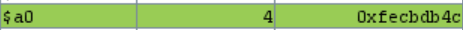
\includegraphics[scale=1]{image/1.2}
	\end{center}
	\item Sau đó, lệnh \colorbox{code}{jal abs} nhảy đến thủ tục abs. Lúc này, thanh ghi \$pc và lệnh tiếp ngay sau câu lệnh \$pc có giá trị 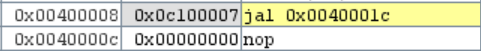
\includegraphics[scale=1]{image/1.3.1}. 
	\item Sau khi thực hiện \colorbox{code}{jal}, thanh ghi \$pc sẽ nhảy đến địa chỉ của thủ tục abs, thanh ghi \$ra lưu giá trị của lệnh ngay bên dưới lệnh \colorbox{code}{jal} 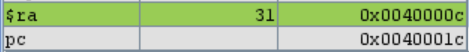
\includegraphics[scale=1]{image/1.4}
	\item \textit{(Ở thủ tục abs, để code hoạt động đúng thì chúng ta phải sao chép giá trị thanh ghi \$a0 vào thanh ghi \$a1 bằng lệnh \colorbox{code}{add \$a1, \$zero, \$a0})}.
	\begin{center}
	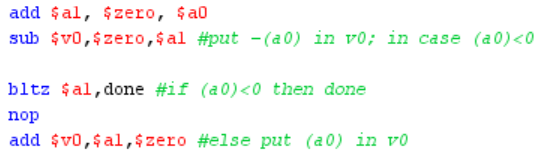
\includegraphics[scale=1]{image/1.3}
	\end{center}
	\item Ở trong thủ tục abs:
		\begin{itemize}
		\item Câu lệnh \colorbox{code}{sub \$v0, \$zero, \$a0} thực hiện gán giá trị -a0 cho thanh ghi \$v0.
		\begin{center}
		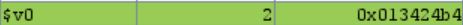
\includegraphics[scale=1]{image/1.5}
		\end{center}
		\item Lệnh \colorbox{code}{bltz \$a1, done} thực hiện so sánh giá trị thanh ghi \$a1 với 0. Nếu \$a1 < 0 thì thực hiện nhảy đến nhãn \textit{done}. \textit{(Thanh ghi \$a1 = -20194484 < 0 nên chương trình sẽ nhảy đến nhãn done, thoát khỏi thủ tục abs)} 
		\end{itemize}	 
	\item Nhãn done chứa câu lệnh \colorbox{code}{jr \$ra}. Khi thực hiện lệnh này, \$pc sẽ nhận giá trị của thanh ghi \$ra.
	\begin{center}
	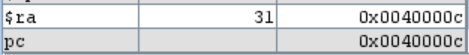
\includegraphics[scale=1]{image/1.6}
	\end{center}
	\item Thực hiện sao chép giá trị thanh ghi \$v0 vào thanh ghi \$s0 bằng câu lệnh \colorbox{code}{add \$s0, \$zero, \$v0}.
	\begin{center}
	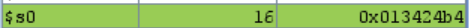
\includegraphics[scale=1]{image/1.7}
	\end{center}
	\item Chương trình kết thúc bằng lời gọi \textit{syscall} với \$v0 = 10.
	\end{itemize}
	\pagebreak
\section*{Assignment 2}
\textbf{Mã nguồn:}
\begin{center}
\begin{lstlisting}
#Laboratory Exercise 7, Home Assignment 2
.text
main: li $a0,4 #load test input
 li $a1,8
 li $a2,4
 jal max #call max procedure
 nop 
 
 add $s0, $zero, $v0
 li $v0,10 #terminate
 syscall 
endmain: 
#---------------------------------------------------------------------

#Procedure max: find the largest of three integers
#param[in] $a0 integers
#param[in] $a1 integers
#param[in] $a2 integers
#return $v0 the largest value
#---------------------------------------------------------------------

max: add $v0,$a0,$zero #copy (a0) in v0; largest so far
 sub $t0,$a1,$v0 #compute (a1)-(v0)
 bltz $t0,okay #if (a1)-(v0)<0 then no change
 nop
 add $v0,$a1,$zero #else (a1) is largest thus far
okay: sub $t0,$a2,$v0 #compute (a2)-(v0)
 bltz $t0,done #if (a2)-(v0)<0 then no change
 nop
 add $v0,$a2,$zero #else (a2) is largest overall
done: jr $ra #return to calling program
\end{lstlisting}
\end{center}
\textbf{Giải thích:}
	\begin{itemize}
	\item 3 câu lệnh đầu tiên thực hiện load 3 giá trị input. \$a0 = 4, \$a1 = 8, \$a2 = 4.
	\begin{center}
	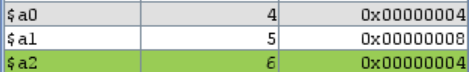
\includegraphics[scale=1]{image/2.1}
	\end{center}
 	\item Lệnh \colorbox{code}{jal max} nhảy đến thủ tục max. Lúc này thanh ghi \$ra lưu giá trị của lệnh kế tiếp lệnh \textit{jal} \quad 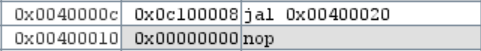
\includegraphics[scale=1]{image/2.2.0}. \\Thanh ghi \$pc nhảy đến địa chỉ của nhãn \textit{max}.
 	\begin{center}
 	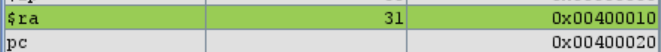
\includegraphics[scale=1]{image/2.2}
 	\end{center}
 	\item Trong thủ tục max:
 	\begin{center}
 	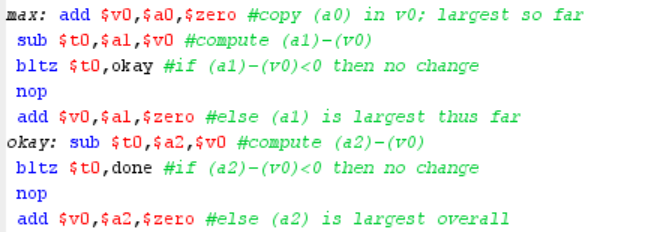
\includegraphics[scale=1]{image/2.3}
 	\end{center}
 		\begin{itemize}
 		\item Đầu tiên, coi \$a0 là giá trị lớn nhất tạm thời bằng cách dùng lệnh \colorbox{code}{add \$v0, \$a0, \$zero}.
 		\begin{center}
 		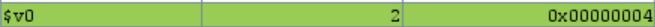
\includegraphics[scale=1]{image/2.4}
 		\end{center}
 		\item Sau đó, dùng lệnh 
 		\item Sau đó, so sánh \$v0 và \$a1 bằng câu lệnh \colorbox{code}{sub \$t0, \$a1, \$v0}. Nếu \$v0 > \$a1 thì rẽ sang nhãn \textit{okay}. Nếu không thì gán giá trị \$a1 là giá trị lớn nhấn tạm thời. \textit{(Ở đây, do \$a0 > \$a1 nên chương trình rẽ sang nhãn okay)}
 		\item Nhãn \textit{okay} thực hiện các bước tương tự, so sánh giá trị lớn nhất tạm thời \$v0 với giá trị của \$a2. Do \$v0 < \$a2 nên thực hiện gán giá trị \$a2 cho thanh ghi \$v0.
 		\begin{center}
 		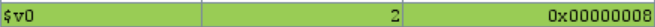
\includegraphics[scale=1]{image/2.5}
 		\end{center}
 		\item Đến nhãn \textit{done}, thủ tục kết thúc. Lệnh \colorbox{code}{jr \$ra} được thực hiện. Thanh ghi \$pc lúc này có giá trị bằng với \$ra.
 		\begin{center}
 		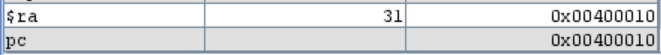
\includegraphics[scale=1]{image/2.6}
 		\end{center}
 		\end{itemize}
 	\item \textit{Ta phải thêm 3 câu lệnh sau vào dưới lệnh mà \colorbox{code}{jr} nhảy đến để chương trình có thể kết thúc được. Giá trị trả về được lưu vào thanh ghi \$s0.}
 	\begin{center}
 	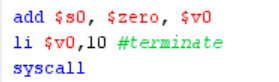
\includegraphics[scale=1]{image/2.7}
 	\end{center}
 	\end{itemize}
 \pagebreak
\section*{Assignment 3}
\textbf{Mã nguồn:}
\begin{center}
\begin{lstlisting}
#Laboratory Exercise 7, Home Assignment 3
.text
addi $s0, $s0, 2019	# $s0 = 4 so dau mssv
addi $s1, $s1, 4484	# $s1 = 4 so cuoi mssv
push: addi $sp,$sp,-8 #adjust the stack pointer
 sw $s0,4($sp) #push $s0 to stack
 sw $s1,0($sp) #push $s1 to stack
work: 
add $s0, $zero, $zero	# $s0 = 0
add $s1, $zero, $zero	# $s1 = 0
pop: lw $s0,0($sp) #pop from stack to $s0
 lw $s1,4($sp) #pop from stack to $s1
 addi $sp,$sp,8 #adjust the stack pointer
\end{lstlisting}
\end{center}
\textbf{Giải thích:}
	\begin{itemize}
	\item 2 câu lệnh đầu tiên thực hiện khởi tạo giá trị cho 2 thanh ghi \$s0 = 2019, \$s1 = 4484.
	\begin{center}
	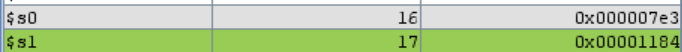
\includegraphics[scale=1]{image/3.1}
	\end{center}
	\item Đến nhãn \textit{push}, ta thực hiện nạp nội dung 2 thanh ghi \$s0, \$s1 vào ngăn xếp. Câu lệnh \colorbox{code}{addi \$s1, \$sp, -8} thực hiện giảm giá trị của thanh ghi \$sp 8 byte. Tạo ra 8 byte trống dùng để lưu 2 biến. (Mỗi biến dùng 4 byte)\\
	Giá trị ban đầu của \$sp:\quad 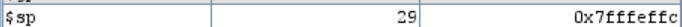
\includegraphics[scale=1]{image/3.2}\\
	Giá trị sau đó của \$sp: \quad 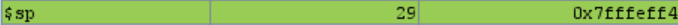
\includegraphics[scale=1]{image/3.3}
	\item 2 câu lệnh \colorbox{code}{sw} tiếp theo dùng để lưu 2 giá trị \$s0, \$s1 vào 2 vị trí chúng ta đã tạo ra trong ngăn xếp.
	\item Đến nhãn \textit{work}, chúng ta thực hiện thay đổi giá trị 2 thanh ghi \$s0, \$s1 thành 0 bằng cách dùng lệnh \colorbox{code}{add \$s0, \$zero, \$zero} và \colorbox{code}{add \$s1, \$zero, \$zero}.
	\begin{center}
	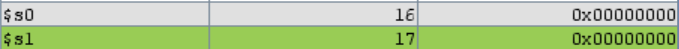
\includegraphics[scale=1]{image/3.4}
	\end{center}
	\item Ở nhãn \textit{pop}, sau khi thay đổi giá trị 2 thanh ghi \$s0, \$s1 về 0, chúng ta tiến hành khôi phục lại giá trị ban đầu bằng cách sử dụng 2 lệnh \colorbox{code}{lw}, load lại dữ liệu đã được lưu trong ngăn xếp vào trong 2 thanh ghi \$s0, \$s1.
	\begin{center}
	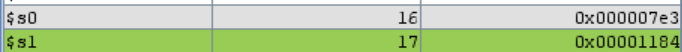
\includegraphics[scale=1]{image/3.1}
	\end{center}
	\item Cuối cùng, thực hiện giải phóng ngăn xếp bằng cách sử dụng lệnh \colorbox{code}{addi \$sp, \$sp, 8}, cộng 8 byte lại cho ngăn xếp.\\
	Giá trị ban đầu của \$sp:\quad 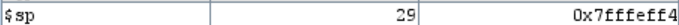
\includegraphics[scale=1]{image/3.5}\\
	Giá trị sau đó của \$sp: \quad 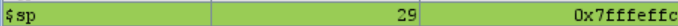
\includegraphics[scale=1]{image/3.6}
	\end{itemize}
\end{document}